\documentclass{BeamerTemplate}
\title{Module 2 - Variables aléatoires à une dimension}
\subtitle{STT-1000 Probabilités et statistique}
\date{\today}

\begin{document}
\begin{frame}[t]
  \titlepage
\end{frame}

\section{Introduction}
\begin{frame}[t]{Exemple 1}
Le résultat d'une expérience aléatoire est souvent un nombre réel, ou encore on assigne une valeur réelle aux résultats possibles d'une expérience.

\medskip
{\ }

\uncover<2->{
% {\bf \underline{Exemple 1}:}\\
 ${\cal E}$: On tire une pièce de monnaie 2 fois
 %et on associe une valeur  réelle $x$ à chaque élément de l'espace échantillonnal

 $\mathcal{U}=\{FF,FP,PF,PP\}$.

 \medskip
 Exemple de valeur associée à chaque résultat: le nombre de fois où Pile apparaît. On peut noter cette variable $X$.

 \begin{tabular}{ll}
 $X=0$  &si le résultat  est $FF$,\\
 $X=1$ &si le résultat est $FP$ ou $PF$,\\
 $X=2$ &si le résultat est $PP$.
 \end{tabular}
}
\end{frame}

\begin{frame}{Variable aléatoire}

Soit $\mathcal{E}$ une expérience aléatoire ayant
  comme espace échantillonnal $\mathcal{U}$.

 \begin{Boite}{Variable aléatoire}
Soit $X$, une fonction  qui associe un nombre réel $X(e)$ à chaque élément
  $e\in \mathcal{U}$. Alors on appelle $X$ une \alert{variable aléatoire}.

\medskip

L'ensemble des valeurs que peut prendre $X$ est noté   $\mathbb{R}_X$ et est appelé \alert{image de $X$}.
 \end{Boite}
On note habituellement une v.a. par une lettre majuscule et les valeurs prises par cette v.a. par une lettre minuscule. On écrira par exemple P(X=x) pour dénoter la probabilité que la variable aléatoire X prenne la valeur x.

\end{frame}

\begin{frame}[t]%{Événements mutuellement exclusifs}

\centerline{\LARGE \bf \alert{QUIZ !}}\label{lancerde}
$\mathcal{E}$: on lance un dé régulier et on observe la face du dessus. \\
$\mathcal{U}=\{1,2,3,4,5,6\}$.\\
On peut définir une infinité de variables aléatoires. \\
Voici 2 exemples.

 \begin{itemize}
  \item<2-> $X$ est la variable aléatoire qui donne le  résultat observé.\\
    $X(e)=e,~\forall e\in \mathcal{U}$\\
    $R_X=\{1,2,3,4,5,6\}$
  \item<3-> Je gagne 1\$ si je roule  4, 5 ou 6.\\
    Je perds 1\$ si je roule 1, 2 ou 3.\\
    $Y$ est la variable aléatoire qui représente mon gain.\\
      $Y(e)=\left\{
  \begin{array}{rl}
  -1 &\text{si}\;e\in\{1,2,3\}\\
  1&\text{si}\;e\in\{4,5,6\}
  \end{array}
  \right.$\\
  $R_Y=\{-1,1\}$.
 \end{itemize}
\end{frame}

\begin{frame}[t]{Exemple 2 (suite)}

\begin{minipage}[b]{4cm}{
{\large

 \begin{tabular}{c|c|c}\hline
 $e$ & $X(e)$ & $Y(e)$ \\ \hline
  1 & & \\
  2 & & \\
  3 & & \\
  4 & & \\
  5 & & \\
  6 & & \\ \hline
 \end{tabular}
}

\vspace{3cm}}
\end{minipage}
\begin{minipage}[b]{6cm}{
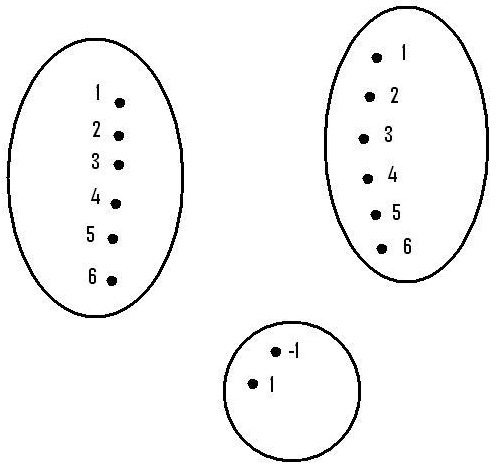
\includegraphics[height=6.8cm]{SmapRxRy-eg.jpg}
}
\end{minipage}
\end{frame}


\begin{frame}[t]{Exemple 2: probabilités}

Quelle est la probabilité que je perde 1 \$ en jouant?\\

%Puisque les événements $A$ et $B$  sont équivalents, leur probabilité est égale. Si le dé est équilibré, quelle est la probabilité que $Y$ prenne la valeur $-1$?

{\large
 \begin{tabular}{c|c|c|c}\hline
 $e$ & $X(e)$ & $Y(e)$ & $P(e)$ \\ \hline
  1 & & & 1/6 \\
  2 & &  & 1/6  \\
  3 & &  & 1/6  \\
  4 & &  & 1/6  \\
  5 & &  & 1/6  \\
  6 & &  & 1/6  \\ \hline
 \end{tabular}
}


\end{frame}

\section{Fonction de répartition}

\begin{frame}{Fonction de répartition}
On peut spécifier complètement le comportement aléatoire de \alerter{toute} variable aléatoire $X$ à l'aide d'une seule fonction.

\begin{defn}{}
Soit $X$ une variable aléatoire. On appelle \alerter{fonction de répartition} (l'acronyme CDF, pour \textit{cumulative distribution function}, est le plus utilisé en pratique), la fonction

$$F_X:\mathbb{R}\to [0,1]$$
qui associe la valeur 
$$F_X(x)=P(X\leq x),$$
à tout $x\in \mathbb{R}$.
\end{defn}
\end{frame}
\begin{frame}[t]{Retour à l'exemple 2}

Quelle est la fonction de répartition du gain $Y$ lors du lancer d'un dé équilibré?%de $Y$?\\

On sait que\\
$\begin{array}{ll}P(Y=-1)&=1/2\\
P(Y=1)&=1/2\end{array}$

\end{frame}

\begin{frame}[t]{Retour à l'exemple 2 (suite)}

 \centerline{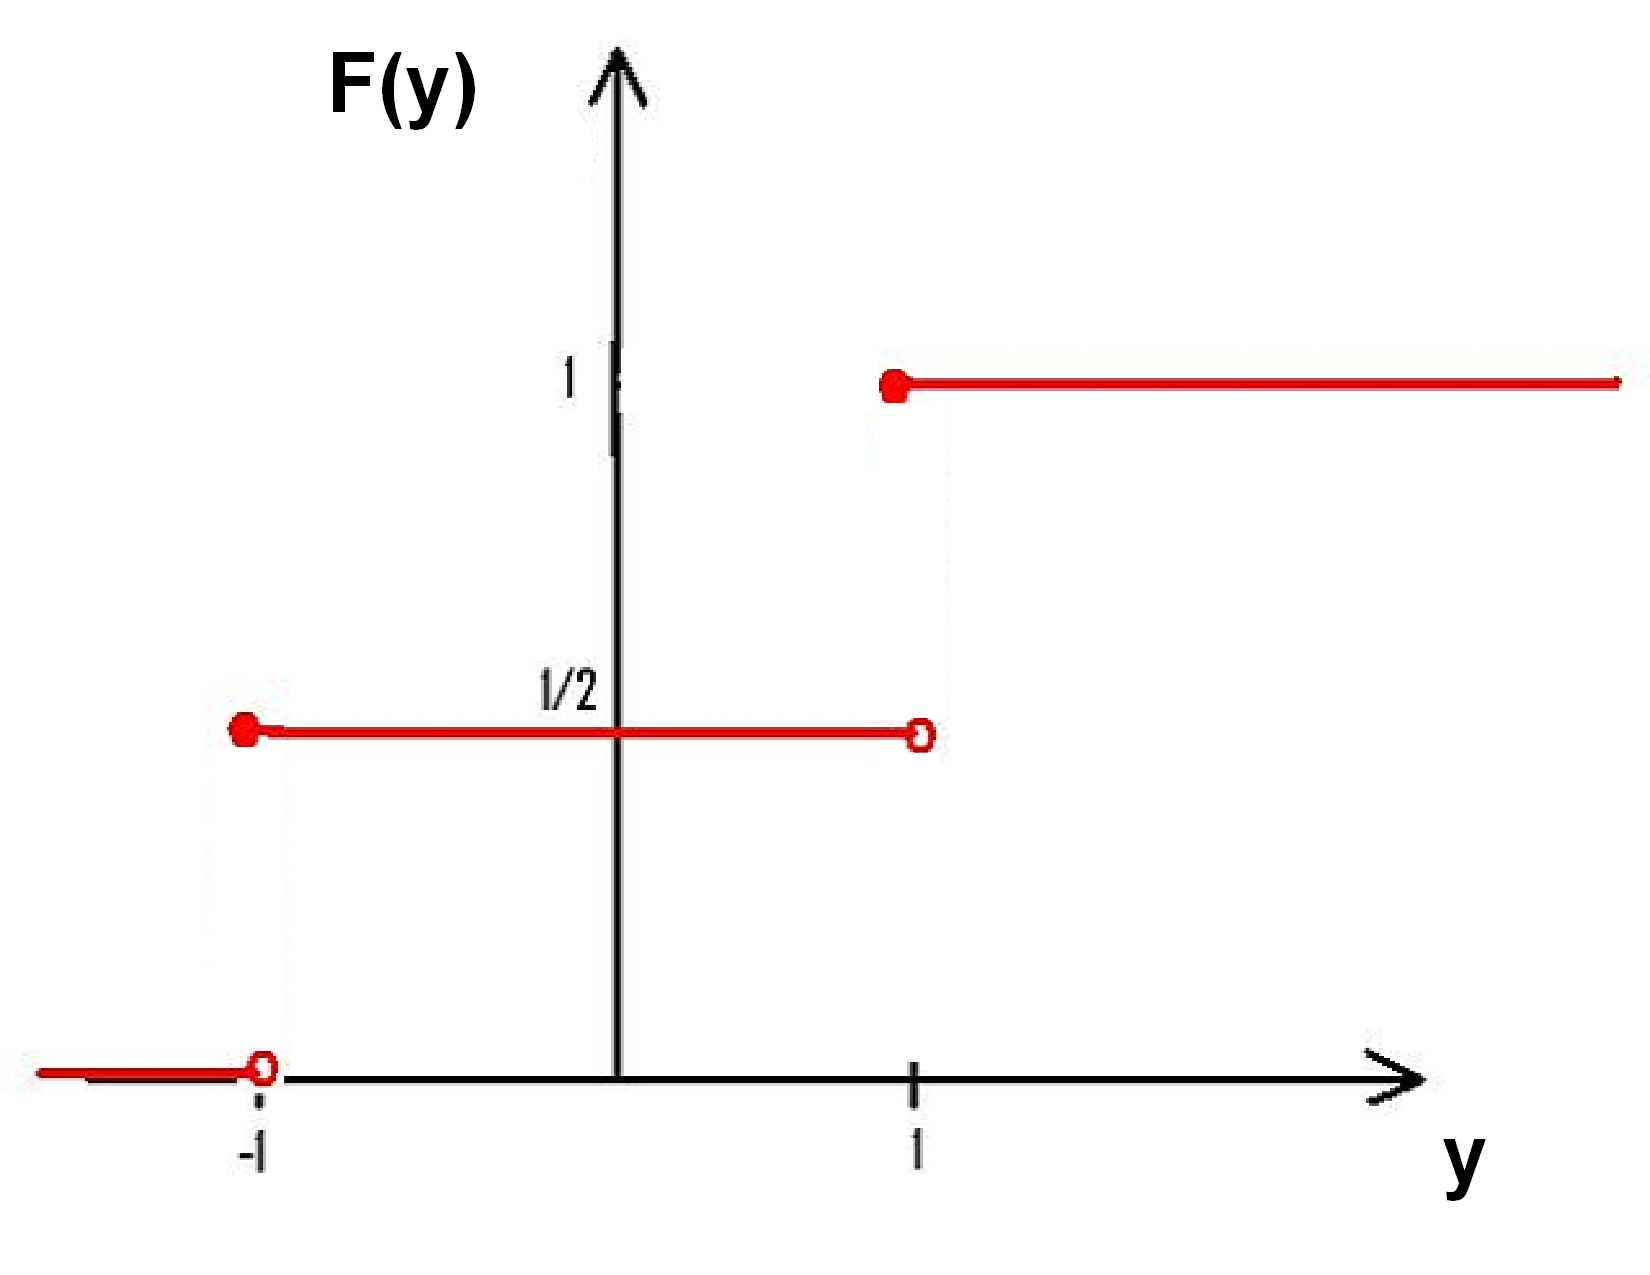
\includegraphics[height=6.8cm]{cdf-modif.pdf}}

\end{frame}

\begin{frame}[t]%{Événements mutuellement exclusifs}

\centerline{\LARGE \bf \alert{QUIZ !}}

{\small %Soit $S=\{u\in\mathds{R}:u\ge0\}$ l'ensemble des quantités possibles de pluie (en mm) à une station météo dans un mois donné. Soit $X(u)=u$, i.e., la v.a. qui représente la quantité de pluie re\c{c}ue.
Soit $X$ la quantité de pluie (en mm) reçue à une station météo dans un mois donné.Un modèle possible pour le comportement aléatoire de $X$ est
 $$F(x)=P(X\le x)=\left\{\begin{array}{ll}
 0 & \textrm{si} \; x<0\\
 1-e^{-\lambda x} & \textrm{si} \; x\ge0,
 \end{array}\right.$$
o\`u $\lambda$ est une constante positive, que l'on suppose connue.}

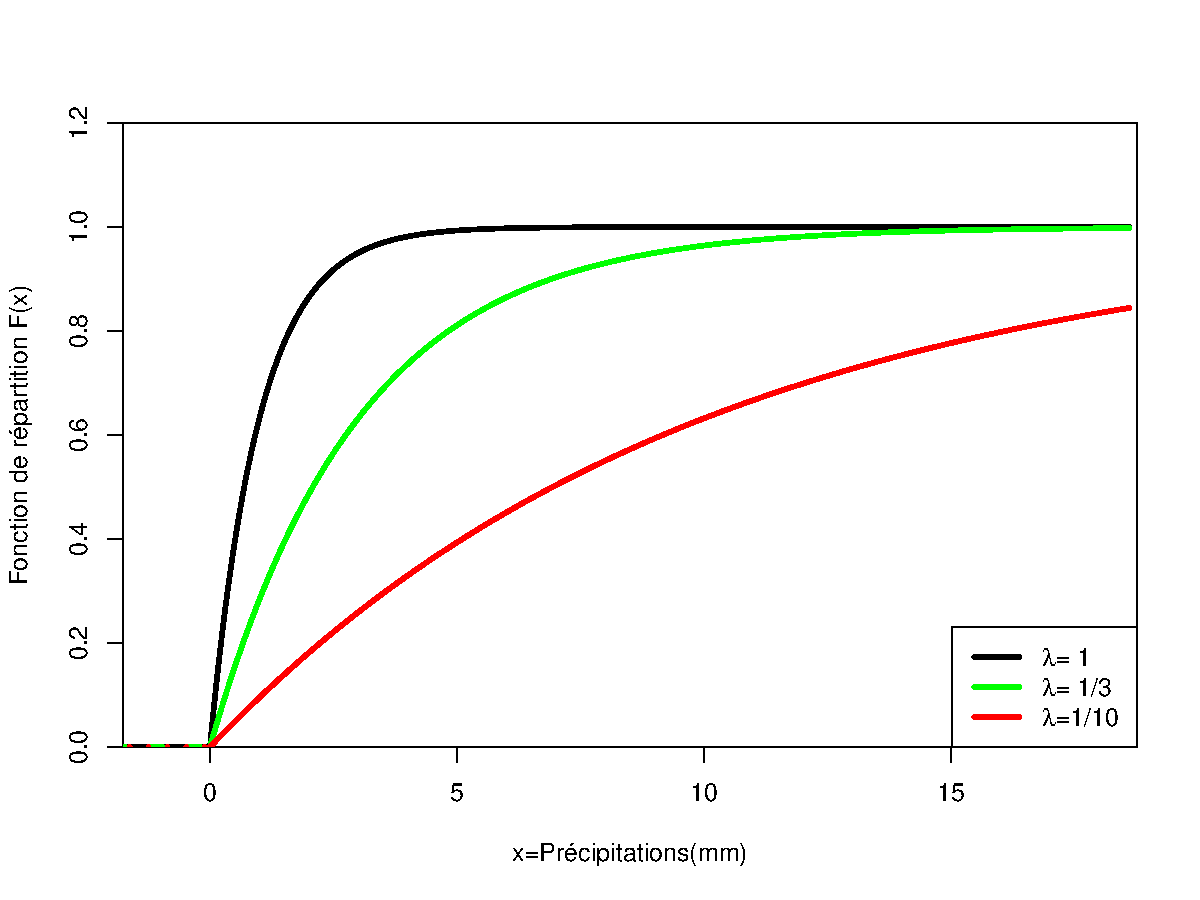
\includegraphics[width=6.2cm]{pluie-repartition.pdf}

\end{frame}
\begin{frame}[t]{Exemple 3 (suite)}

Supposons que $\lambda=1/10$. Calculez ces probabilités.

\begin{itemize}\itemsep=12mm
\item $P(X\leq 15)$
\item $P(X> 10)$
\item $P(5<X\leq 10)$
\end{itemize}

\vspace{5mm}
\end{frame}


\begin{frame}[t]%{Événements mutuellement exclusifs}

\centerline{\LARGE \bf \alert{QUIZ !}}
Quelle est la probabilité d'obtenir un gain supérieur à 0,75\$ ?

\medskip
Répondez à l'aide de la fonction de répartition.

\vspace{5cm}

\end{frame}


\begin{frame}[t]{Propriétés d'une fonction de répartition}

{\small
\begin{itemize}
 \item[1.] $0\le F_X(x)\le 1$ pour tout $x\in\mathbb{R}$
 \item[2.] $\lim\limits_{x\to\alerter{-\infty}}F_X(x)=0$ et $\lim\limits_{x\to\alerter{\infty}}F_X(x)=1$
 \item[3.] $F_X(x)$ est \alerter{non décroissante} (si $x_1\le x_2$, alors $F_X(x_1)\le F_X(x_2)$)
 \item[4.] $F_X(x)$ est \alerter{continue à droite}, $\left(\lim\limits_{s\to 0+}F_X(x+s)=F_X(x),\;\forall x\in\mathbb{R}\right)$
\end{itemize}

\uncover<2->{
 \begin{itemize}
  \item Pour vérifier si une fonction est une fonction de répartition,   on vérifie si elle remplit les 4 propriétés ci-dessus.
  \item De la définition d'une fonction de répartition, on a que  pour tout $a<b$, $P(a<X\le b)=F_X(b)-F_X(a)$.
 \end{itemize}
}
}
\end{frame}

\begin{frame}

\begin{block}{Variables aléatoires discrètes et continues}
\begin{itemize}\itemsep3mm
\item  Si $F_X(x)$ est une fonction en escalier continue à droite,  alors on dit que $X$ est une variable aléatoire \alerter{discrète}. L'ensemble des valeurs possibles est \alerter{dénombrable}.
\item Si $F_X(x)$ est une fonction continue, alors on dit que  $X$ est une variable aléatoire \alerter{continue}. L'ensemble des valeurs possibles est \alerter{indénombrable}
 \end{itemize}
\end{block}


\end{frame}

\section{Variables aléatoires discrètres}

\begin{frame}[t]{Fonction de probabilité/masse}

 \begin{defn}
  Soit $X$ une v.a. \alerter{discrète}. On  appelle \alerter{fonction de probabilité} (ou \alerter{fonction de masse},
  ou \alerter{fonction de masse de probabilité}. On utilise PMF, de \textit{probability mass function}) de $X$ la fonction
  $$p_X:\mathbb{R}\to[0,1]$$ qui associe la valeur 
  $$p_X(x)=P(X=x)$$
  à tout $x\in \mathbb{R}$.
 \end{defn}
 
\end{frame}




\begin{frame}{Exemples}

\vspace{-1.5 in}
Retournons à l'exemple du dé.\\
Trouvons $p_X$ et $p_Y$.


\end{frame}


\begin{frame}{Exemples - suite}




\end{frame}



\begin{frame}[t]{Propri\'et\'es de la fonction de probabilit\'e}

Une fonction $p_X$ peut être une fonction de probabilité pour une v.a. discrète $X$ \alerter{si et seulement si} elle satisfait deux propriétés:

\vspace{0.2 in}

\begin{enumerate} 
 \item $ $
 \vspace{0.3 in}
 \item $ $
\end{enumerate}

\end{frame}

\section{Variables aléatoires continues}

\begin{frame}[t]{Fonction de densité}

\begin{defn}
Soit $X$ une v.a. continue. On appelle fonction de densité (PDF, de \textit{probability density function}) de $X$, la fonction qui associe la valeur 
$$f_X(x)=\frac{d}{dx}F_X(x)$$
à tout $x\in \mathbb{R}$.
\end{defn}
\end{frame}
\begin{frame}

\begin{Boite}{Lien entre la fonction de répartition $F_X(x)$ et la fonction de densité $f_X(x)$}
Par la définition de la fonction de densité $f_X(x)$, on remarque:
\begin{align*}
 F_X(x)&=\int_{-\infty}^x f_X(u)\;du \\
 P(a<X\le b)&=F_X(b)-F_X(a)=\int_a^bf_X(u)\;du.
\end{align*}
On en déduit donc que la probabilité d'une variable aléatoire continue peut se calculer avec l'intégrale de $f_X(x)$.
\end{Boite}

\end{frame}

\begin{frame}[t]{Probabilité = aire sous la densité}

\centerline{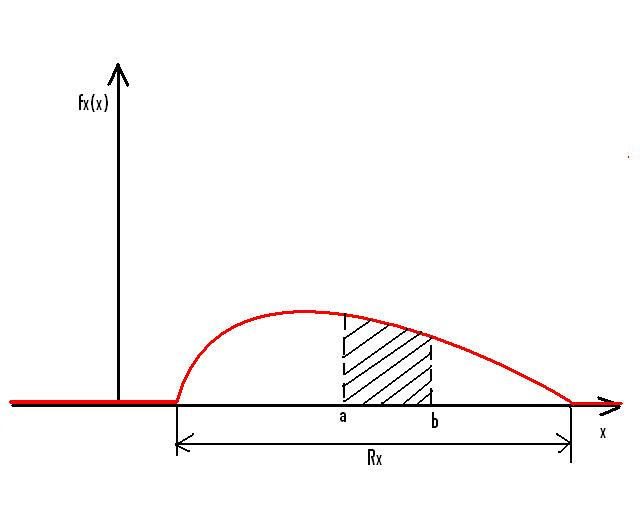
\includegraphics[height=1.65in]{pdf-aire.jpg}}

$f_X(x)$ n'est \alerter{pas} une probabilité, mais son intégrale sur une région donne la
probabilité que $X$ prenne une valeur dans cette région.

Ceci veut dire que $f_X(x) \alerter{\neq} P(X=x)$.

\end{frame}

\begin{frame}[t]{Propriétés d'une fonction de densité}

\begin{itemize}
 \item[1.] $f_X(x)\ge0$ pour tout $x\in\mathbb{R}$
 \item[2.] $\displaystyle\int_{-\infty}^\infty f_X(x)\;dx=1$
 \item[3.] $f_X(x)$ est continue par morceaux
 \item[4.] si $x\notin \mathbb{R}_X$, alors $f_X(x)=0$ %(et donc  $\int_{-\infty}^\infty f(x)\;dx=1$)
\end{itemize}

\uncover<2->{
Comme $\displaystyle\int_a^af_X(u)\;du=0$,
alors $P(X=a)=0$ pour tout $a\in\mathbb{R}$ dans le cas
d'une v.a. \underline{continue}. Ceci implique que
$$
\left.\begin{array}{l}
P(a<X<b)\\P(a<X\le b)\\P(a\le X<b)\\P(a\le X\le b)
\end{array}\right\}=\int_a^bf_X(u)\;du.$$}

\end{frame}

\begin{frame}[t]%{Événements mutuellement exclusifs}

\centerline{\LARGE \bf \alert{QUIZ !}}

{\small
Soit une v.a. $X$ continue pouvant prendre toute valeur dans l'intervalle
$[0,20]$. On vous dit que
\begin{itemize}
\item tous les intervalles de même longueur dans $[0,10)$ sont équiprobables,
\item tous les intervalles de même longueur dans $[10,20]$ sont équiprobables,
\item tous les intervalles dans $[10,20]$ est deux fois plus probable qu'un intervalle de même longueur dans $[0,10)$.
    \end{itemize}
Déterminez la densité de $X$, sa fonction de répartition, et évaluez $P(5<X<12)$.}
\end{frame}


\begin{frame}[t]{Exemple 5: Retour à l'exemple de la pluie}
La distribution de la quantité de pluie mensuelle re\c{c}ue à la station
est définie par $F(x)=1-e^{-\lambda x}$ si
$x\ge0$, et $0$ ailleurs.
\begin{itemize}\itemsep 2cm
\item Quelle est la densité de $X$?
\item Quelle est la probabilité que la quantité de pluie re\c{c}ue excède 5 mm?
%\item Quelle est la probabilité de recevoir entre 10 et 15 mm sachant que l'on recevra au moins 5 mm?
\end{itemize}
\end{frame}

\begin{frame}[t]%{Événements mutuellement exclusifs}

\centerline{\LARGE \bf \alert{QUIZ !}}
\begin{itemize}
\item Quelle est la probabilité de recevoir entre 10 et 15 mm sachant que l'on recevra au moins 5 mm?
\end{itemize}

\end{frame}


\begin{frame}[t]%{Événements mutuellement exclusifs}

\centerline{\LARGE \bf \alert{QUIZ !}}
Associez chaque densité  avec la bonne répartition.
\begin{center}
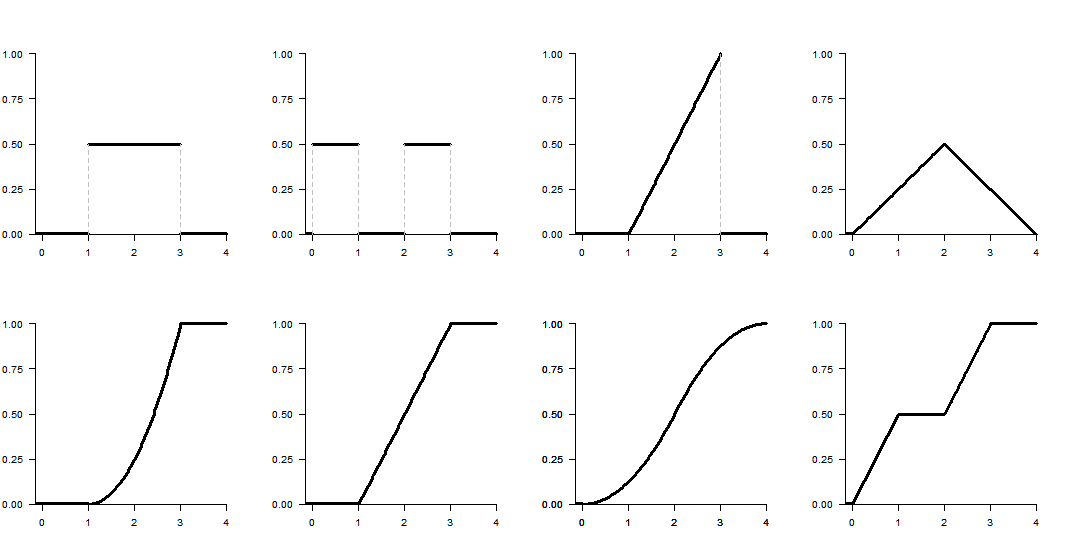
\includegraphics[width=12cm]{association.png}
\end{center}

\end{frame}

\section{Espérance et variance d'une variable aléatoire}

\begin{frame}[t]{Aspects importants d'une distribution}
Même si les fonctions de répartion, de densité ou de probabilité spécifient complètement la distribution d'une variable aléatoire, il est utile de s'intéresser aux caractéristiques qui résument les aspects
principaux de son comportement:

\medskip
\begin{itemize}\itemsep2mm
\item tendance centrale;
\item dispersion;
\item forme.
\end{itemize}

Notez qu'à partir de maintenant, quand il n'y aura qu'une seule variable aléatoire à l'étude, nous écrirons $F(x)$, $p(x)$ et $f(x)$ au lieu de $F_X(x)$, $p_X(x)$ et $f_X(x)$.

\end{frame}

\begin{frame}[t]{Mesure de la tendance centrale}
\begin{defn}
 L'\alerter{espérance} (moyenne théorique) d'une variable aléatoire $X$ est donnée par
  $$
 E(X)=\sum_{x\in \mathbb{R}_X} x p(x)$$
 pour une variable aléatoire...\\
 
 ou 
 $$
 E(X)=\int_{-\infty}^\infty xf(x)\;dx.$$
pour une variable aléatoire...\\

\end{defn}
La notation la plus fréquente est $E(X)=\mu$.
\end{frame}

\begin{frame}[t]{Interprétation de l'espérance de X}
    C'est la valeur moyenne que l'on obtiendrait si on réalisait l'expérience aléatoire une infinité de fois. 
    
\vspace{1cm}

    Pour une variable aléatoire continue, en pratique, nous n'observerons jamais une moyenne sur un nombre fini d'expériences aléatoires exactement égale à l'espérance.
    
\vspace{1cm}

    Ceci n'est pas tout à fait vrai pour une variable aléatoire discrète. Un exemple?
\end{frame}

\begin{frame}[t]{Exemple 6: Retour à l'exemple de la pluie}
\begin{minipage}[b]{4.2cm}{
 {\small $f(x)=\left\{\begin{array}{c l}\lambda e^{-\lambda x}&\text{si} \;x>0\\
 0&\text{si} \; x\leq 0
 \end{array}\right.$

\vspace{3mm}

Quelle quantité de pluie tombe-t-il en moyenne durant ce mois? (Répondez pour $\lambda$ en général, sans fixer de valeur).
}

 \vspace{3mm}

 $\mbox{ }$ }
 \end{minipage}\hspace{4mm}
 \begin{minipage}[t]{6cm}{
 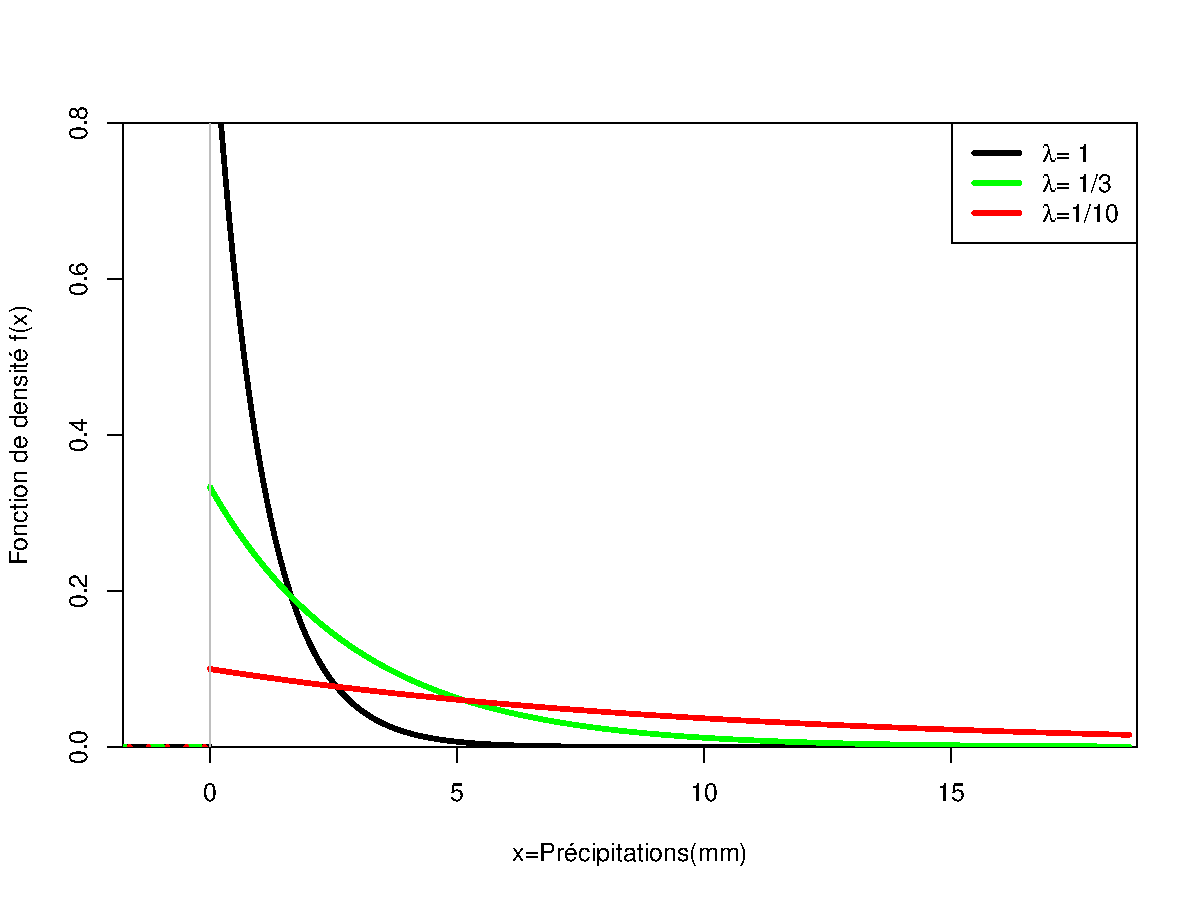
\includegraphics[width=6cm]{pluie-densite.pdf}}
 \end{minipage}

 %\vspace{-3cm}
 %Quelle quantité de pluie tombe-t-il en moyenne durant ce mois? (Répondez pour $\lambda$ en général, sans fixer de valeur).

\end{frame}

\begin{frame}[t]{Variabilité d'une variable aléatoire}

Deux variables aléatoires peuvent avoir la \underline{même espérance},
 mais l'une peut être beaucoup \underline{plus variable
 que l'autre}, i.e., avoir tendance à prendre des valeurs
 plus éloignées de son espérance que l'autre.

 \medskip
 {\bf \underline{Expérience}:} Rouler 30 dés réguliers.

 $X_1=$ la valeur indiquée par le premier dé\\
 $X_2=$ la moyenne des 30 dés (la somme divisée par 30).

 \medskip
 On peut montrer que $X_1$ et $X_2$ ont la m\^eme
 espérance ($3,5$).

 \medskip
 Cependant, $X_2$ aura tendance à prendre
 des valeurs très proches de $3,5$, alors que $X_1$ peut prendre
 n'importe quelle valeur entre 1 et 6 avec la m\^eme probabilité.

\end{frame}

\begin{frame}[fragile]
\frametitle{Petite simulation}
{\small
Voici un exemple où on a simulé 12
fois l'expérience à l'aide de \texttt{R}:

\begin{verbatim}
      X1            X2
 [1,]  2       3.633333
 [2,]  6       3.666667
 [3,]  4       3.933333
 [4,]  4       3.633333
 [5,]  5       3.833333
 [6,]  6       3.600000
 [7,]  6       3.400000
 [8,]  3       3.166667
 [9,]  2       3.766667
[10,]  5       3.066667
[11,]  3       3.566667
[12,]  1       3.300000
\end{verbatim}
}
\end{frame}

\begin{frame}[t]{Fonctions de probabilité de $X_1$ et $X_2$}

{\small La figure ci-dessous montre la fonction de probabilité de $X_1$
en bleu et celle de $X_2$ en rouge. M\^eme si les deux v.a. ont la m\^eme
moyenne, on voit bien que la distribution de $X_2$ est beaucoup
plus concentrée autour de 3,5 que celle de $X_1$.

\centerline{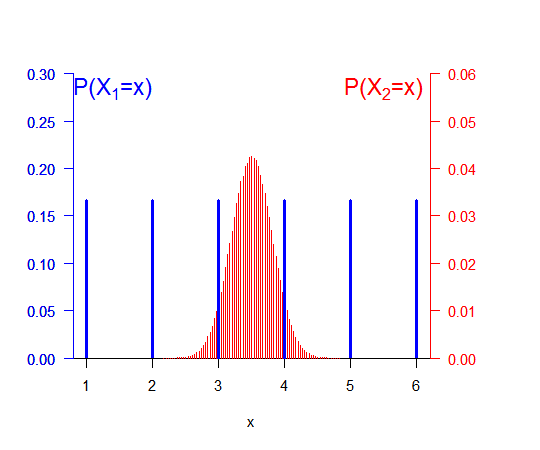
\includegraphics[height=2.1in]{pmf-x1x2-modif.png}}

%(Note: Pour $P(X_2=x)$, les barres rouges ne sont pas à l'échelle et n'apparaissent pas pour toutes les valeurs de $R_{X_2}$.)
}
\end{frame}

\begin{frame}[t]{Mesure de dispersion d'une distribution}

\begin{defn}
La \alerter{variance} d'une variable aléatoire $X$ est donnée par
  $$V(X)=\sum_{x\in \mathbb{R}_X} (x-\mu)^2p(x)$$
pour une variable aléatoire discrète et
  $$V(X)=\int_{-\infty}^\infty (x-\mu)^2f(x)\;dx.$$
pour une variable aléatoire continue.
\end{defn}
La notation la plus fréquente est $V(X)= \sigma^2$.

Une quantité très utile qui découle de la variance est l'écart-type, $\sigma = \sqrt{V(X)}=\sqrt{\sigma^2}$.

\end{frame}


\begin{frame}[t]{Exemple 7: Retour à l'exemple de la pluie}

La quantité de pluie reçue en un mois à cette station est-elle très variable?
\end{frame}

\section{Espérance mathématique d'une fonction de variable aléatoire}

\begin{frame}[t]{Valeur espérée d'une fonction de $X$}

{\small
\begin{Boite}{Espérance mathématique d'une fonction de $X$}
 Soit $X$ une v.a. et posons $Y=H(X)$ une fonction
 de $X$. Alors l'\alert{espérance mathématique
 de $H(X)$} (ou de $Y$) est définie par
 $$E[Y]=E[H(X)]=\sum_{x\in\mathbb{R}_X}H(x)p(x)$$
 ou
 $$E[Y]=E[H(X)]=\int_{-\infty}^\infty H(x)f(x)\;dx.$$
\end{Boite}
Un cas particulier...
\begin{itemize}
 \item $H(X)=(X-\mu)^2\Rightarrow E[(X-\mu)^2]=V[X]=\sigma^2=\;\;$variance de $X$.
\end{itemize}
}
\end{frame}

\begin{frame}[t]{Résultats utiles}

Supposons que $a$ et $b$ sont des constantes.

\begin{itemize}
\item<1-> $E[aX+b]=aE[X]+b$\ \ \ \ \
%\underline{Preuve}:

\vspace{0.45in}

\item<1-> $V[X]=E[X^2]-(E[X])^2$\ \ \ \ \
%\underline{Preuve}:

\vspace{0.75in}

\item<1-> $V[aX+b]=a^2V[X]$\ \ \ \ \
%\underline{Preuve}:
\end{itemize}
\end{frame}

\begin{frame}[t]
Prouvez $E[aX+b]=aE[X]+b$ dans le cas d'une variable aléatoire continue.

\end{frame}

\begin{frame}[t]
Prouvez $V[X]=E[X^2]-(E[X])^2$.

\end{frame}

\begin{frame}[t]
Prouvez  $V[aX+b]=a^2V[X]$.

\end{frame}

\begin{frame}[t]{Exemple 8: Retour à l'exemple de la pluie}

Supposons que les revenus (en centaines de milliers de dollars)
générés par un barrage sont bien modélisés par l'équation $R=10+3X$ (où $X$ est la quantité de pluie). Quelle est la valeur
moyenne et l'écart-type de ces revenus?

Rappel: $E(X)=1/\lambda\qquad V(X)=1/\lambda^2$
\end{frame}



\begin{frame}{Bibliographie}
 	Ce document est rédigé avec Beamer ainsi qu'une classe .cls fourni par Jérôme Soucy. Les diapositives sont adaptées des diapositives créées par Anne-Sophie Charest 
 pour le cours STT-1000 ainsi que celles créées par Thierry Duchesne et Emmanuelle Reny-Nolin pour le cours STT-1900.
 	\printbibliography
 	\vfill
 	\footnotesize Pour signaler une erreur dans ce document, veuillez écrire à l'adresse :~\href{mailto:julien.miron@mat.ulaval.ca}{julien.miron@mat.ulaval.ca}.
 \end{frame}

\end{document}

